\subsection{Background}
\begin{frame}
	\frametitle{Background}
	\begin{itemize}
		\item France - preparation for a transition from LWRs to SFRs \cite{noauthor_cne2_nodate}
		\item France - additional LWR construction to supply Plutonium for SFR transition
		\item Most EU nations do not have a repository for UNF
	\end{itemize}
\end{frame}

\begin{frame}
	\frametitle{Abstract}
	By taking UNF from other EU nations, France can transition into a fully SFR fleet (66 GWe)
	without additional construction of LWRs.
	\begin{itemize}
		\item 66 GWe -> 110 ASTRID-type SFRs
		\item Collaborative approach seeks to benefit both sides
	\end{itemize}
\end{frame}

\begin{frame}
	\frametitle{Literature Review}
	\begin{itemize}
		\item French transition into SFR after additional construction of EPRs 	
		\cite{carre_overview_2009, martin_symbiotic_2017, freynet_multiobjective_2016}
		\item partitioning and transmutation in a regional (European) context \cite{fazio_study_2013}
	\end{itemize}
\end{frame}

\subsection{Method and Specfications}

\begin{frame}
	\frametitle{Method}
	\Cyclus, the agent-based simulator \cite{huff_fundamental_2016} is used.
	Two simulations are run:
	\begin{itemize}
		\item EU UNF inventory at 2050 (1970-2050)
		\item French transition to SFRs (1970-2160)
	\end{itemize}
	The UNF and tails inventory from the first simulation is used for the second simulation.
\end{frame}

\begin{frame}
	\frametitle{Deployment Timeline for EU historical operation}
	Historical operation and predictions are made using references such as IAEA PRIS \cite{iaea_pris_nodate},
	World Nuclear Association \cite{world_nuclear_association_nuclear_2017} and other papers
	\cite{joskow_future_2012, hatch_politics_2015}.
	\begin{figure}[htbp!]
		\begin{center}
			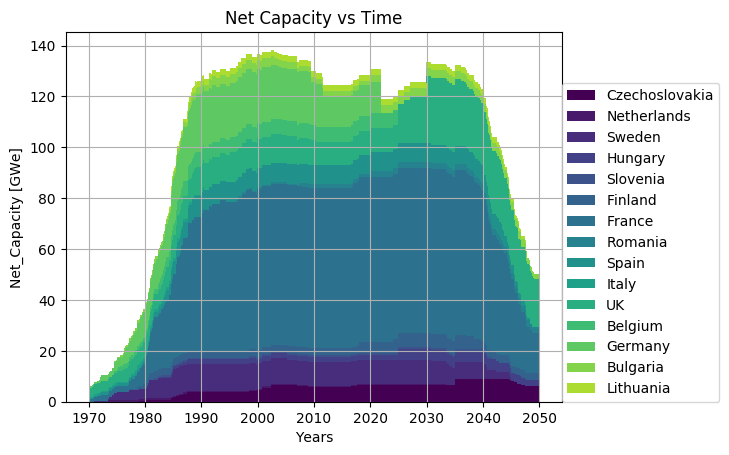
\includegraphics[width=.8\linewidth,height=.8\textheight,keepaspectratio]{./images/eu_future/power_plot.png}
		\end{center}
		\caption{Timeseries of installed nuclear capacity in \gls{EU}.}
		\label{fig:eu_pow}
	\end{figure}
	
\end{frame}

\begin{frame}
	\frametitle{Deployment Timeline for French Transition}
	600 MWe SFRS are deployed to a capacity of 66,000 MWe by 2076.
	\begin{figure}[htbp!]
	\begin{minipage}[b]{.45\linewidth}
        \begin{center}
                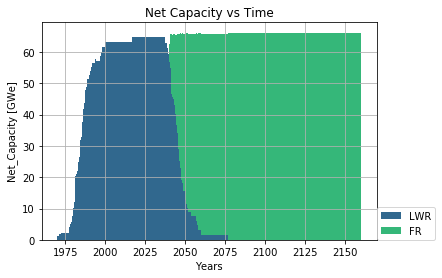
\includegraphics[width=\textwidth]{./images/french-transition/power_plot.png}
        \end{center}
        \caption{French Transition into an SFR Fleet}
        \label{fig:sfr_num}
	\end{minipage}
	\hspace{.5cm}
	\begin{minipage}[b]{.45\linewidth}
		\centering
		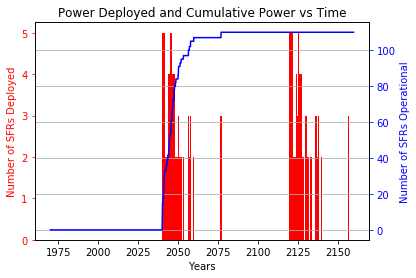
\includegraphics[width=\textwidth]{./images/french-transition/sfr_deploy.png}
		\caption{Deployment of French \glspl{SFR} and total installed capacity}
		\label{fig:dep}
	\end{minipage}
\end{figure}
\end{frame}